\chapter{Traveling Salesman}
The Traveling Salesman Problem, or TSP is a widely studied $\nph{}$ combinitorial optimization problem in which the decision version of the problem is $\npc{}$. Intuitively, TSP is a problem in which we are given a set of cities and the distances between each pair of cities, and we aim to find the shortest possible route that visits each city exactly once and returns to the starting city. Formally, though, we define it as such:
\begin{definition}[Traveling Salesman Problem]
Given a complete weighted graph $G = (V, E)$, where each edge $(u, v) \in E$ has a non-negative weight $w(u, v)$, find a Hamiltonian cycle (a tour that visits each vertex exactly once) $T$ of minimum total weight.
\end{definition}  

Note that many definitions of TSP use an undirected graph, where if there is an edge $(u,v)$ there must also be an edge $(v,u)$. Originally, we used this definition as well, but we discovered a conversion from directed graphs to undirected graphs that preserves the structure of any Hamiltonian cycles, allowing us to instead focus on directed graphs, as any proofs would carry over. This conversion can be seen in Jonker and Volgenant's work \cite{JONKER1983161}.

We must also formally define our various second-best problems here, and they will be applied across multiple restrictions on the standard travelling salesman problem.

\begin{definition}[\exob{}-TSP]
Given an instance of the Traveling Salesman Problem and an optimal tour $T$, find a tour $T'$ such that $w(T') > w(T)$ and no tour $T''$ exists with $w(T) < w(T'') < w(T')$, where $w(T)$ denotes the total weight of tour $T$.
\end{definition}

\begin{definition}[\inob{}-TSP]
Given an instance of the Traveling Salesman Problem and an optimal tour $T$, find a tour $T' \neq T$ such that $w(T') \geq w(T)$ and no tour $T'' \neq T$ exists with $w(T) \leq w(T'') < w(T')$.
\end{definition}

\begin{definition}[\exb{}-TSP]
Given an instance of the Traveling Salesman Problem, find a tour $T'$ such that $w(T') > w(T)$, where $T$ is an optimal tour, and no tour $T''$ exists with $w(T) < w(T'') < w(T')$.
\end{definition}

As noted in our introduction, we will not be handling \inb{} problems due to the lack of a conclusive definition.

\section{Unrestricted TSP}
In future sections, we will restrict the types of graphs that are permitted as inputs in order to make the problems computationally easier to solve and therefore potentially more interesting for our purposes, however we begin with an unrestricted form of the Traveling Salesman. For our first result, we will prove the following:

\begin{theorem}
    \inob{}-TSP is $\nph{}$
\end{theorem}

This result uses a technique first used by Papadimitriou and Steiglitz in their proof that it is impossible to determine whether a graph has a Hamiltonian cycle given an example of a Hamiltonian path in the graph \cite{nphard}. This is an interesting result in its own right, because one might expect that, given a Hamiltonian path -- a sequence of neighboring vertices that includes every vertex in the graph -- one would be able to also find a Hamiltonian cycle, which has the same definition except it must start and end at the same vertex. 
% The proof uses a directed graph, however converting a directed graph to an undirected graph for the traveling salesman problem is a known process. We can use the process described by Jonker and Volgenant to produce an undirected graph with double the number of vertices but in which the optimal (and as it is easy to show), second-best solution is maintained \cite{JONKER1983161}. 


To prove our theorem, we will use a reduction from unrestricted TSP to our \exob{}-TSP. First, let us define a special graph, $H$ first used in \cite{nphard}. We will use a diagram to define $H$ in \autoref{hgraph}, but it is important to note that the specific shape of the graph is not necessary to its construction, only the vertices and the edges connecting them.
\begin{figure}[!ht]
	\centering
	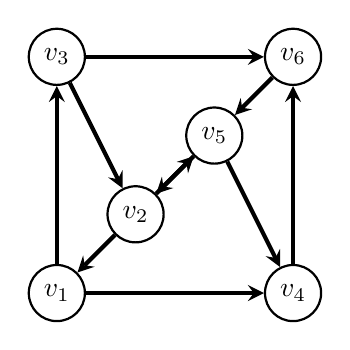
\begin{tikzpicture}[>=stealth, ->, thick, node distance=2.5cm]
	    \node[circle, draw] (v1) at (0,0) {$v_1$};
	    \node[circle, draw] (v2) at (1,1) {$v_2$};
	    \node[circle, draw] (v3) at (0,3) {$v_3$};
	    \node[circle, draw] (v4) at (3,0) {$v_4$};
	    \node[circle, draw] (v5) at (2,2) {$v_5$};
	    \node[circle, draw] (v6) at (3,3) {$v_6$};
	    
	    \draw[->, line width=1.5pt] (v1) -- (v3);
	    \draw[->, line width=1.5pt] (v1) -- (v4);
	    \draw[->, line width=1.5pt] (v3) -- (v6);
	    \draw[->, line width=1.5pt] (v3) -- (v2);
	    \draw[->, line width=1.5pt] (v6) -- (v5);
	    \draw[->, line width=1.5pt] (v2) -- (v5);
	    \draw[->, line width=1.5pt] (v5) -- (v4);
	    \draw[->, line width=1.5pt] (v5) -- (v2);
	    \draw[->, line width=1.5pt] (v4) -- (v6);
	    \draw[->, line width=1.5pt] (v2) -- (v1);
	\end{tikzpicture}
	\caption{Digraph $H$.}\label{hgraph}
\end{figure}
Let us also acknowledge a lemma proven by Papadimitriou and Steiglitz in \cite{nphard}.
\begin{lemma*}
    Let the graph $H$ (\autoref{hgraph}) be a subgraph of another graph $G$ such that edges of $G - H$ enter $H$ only at $v_1$ or $v_3$ and leave $H$ only at $v_4$ or $v_6$. Then, if $G$ has a hamiltonian cycle $T$, exactly one of the paths $(v_1, v_3, v_2, v_5, v_4, v_6)$  or $(v_3,v_6,v_5,v_2,v_1,v_4)$ is a part of $T$.
\end{lemma*}
The proof of this lemma is quite interesting in its own right and is one of many reasons it is worth it to read \cite{nphard}, but we will only give a brief outline rather than proving the result. First, we limit the input edges from the graph outside of $H$, that is, $G-H$, to only enter at $v_1$ or $v_3$ and leave from $v_4$ or $v_6$. We also note that any Hamiltonian cycle in the graph must include every vertex in $H$. Thus, if we enter $H$ from $v_1$, the only option that makes it possible to include every vertex in $H$ is to leave through $v_6$ (through the first path in the lemma). On the other hand, if we enter from $v_3$, the only option is to leave through $v_4$, the second path in the lemma. These can be seen by attempting to path through $H$ in any other way and realizing it is impossible to reach every vertex. This allows us to essentially control where in a subgraph we exit from based on where we entered.

Let us now use $H$ to prove the hardness of \inob{}-TSP. 
Given an instance of the original traveling salesman problem with inputs $G = (V,E)$, we will construct a new graph $G' = (V', E')$ using the following steps:
\begin{enumerate}
    \item For every vertex $u \in V$, create a new instance of $H$, $H_u$ with vertices $\{v_1^{u}, ..., v_6^{u}\}$. We define $V'$ as $V' = \{v_i^u : 1 \leq i \leq 6, u \in V\}$.
    \item For every instance of $H_u$ in $V'$, we create edges between each $v_i^u$ as expected from our original definition of $H$, each with a weight of $0$. For instance, we have an edge $(v_1^u, v_4^u)$. We include these edges in $E'$. 
    \item For every edge $(u_1,u_2) \in E$, we create an edge from $v^{u_1}_4$ to $v^{u_2}_3$ with weight $w(u_1,u_2)$. We also include these edges in $E'$.
    \item Arbitrarily assign each instance of $H$ a number, $H_1,..., H_n$ where $n$ is the number of vertices in $V$. Then, for each $H_i$, we add an edge $(v_6^i,v_1^{i+1})$. We also add the edge $(v_6^n, v_1^1)$. We give each of these edges a weight of $0$. We include these edges in $E'$.
\end{enumerate}

We will show that the solution to \inob{}-TSP on input $G' = (V', E')$ with provided optimal solution $T = (H_1, ..., H_n, H_1)$ (here we slightly abuse the notation by showing a sequence of subgraphs rather than sequence of vertices, but the meaning is clear -- in the real input we would have to replace each of the $H_i$ with its respective sequence of $v_j^i$ vertices, specifically in the path $(v_1, v_3, v_2, v_5, v_4, v_6)$) is exactly the solution to the original TSP instance.

First, we must show that $T$ is an optimal solution itself. Since the weight of each edge in the traveling salesman problem is nonnegative, we know that the total weight of any Hamiltonian cycle must also be nonnegative. Thus, the lowest possible weight for such a cycle must be $0$. Since we set the weight of each $(v_6^i,v_6^{i+1})$ and $(v_6^n, v_1^1)$ to $0$, $w(T)$, the total weight of $T$, must be $0$. Additionally, $T$ must be a Hamiltonian cycle, as it includes every vertex in every instance of the $H$ subgraph, which is by definition the entirety of $V'$. Thus, $T$ is an optimal Hamiltonian cycle for $G'$. Now, we will show that the solution to \inob{}-TSP on $G'$ gives us the exact solution to the original TSP on graph $G$. We will consider solutions to be unique up to cyclical rotation. That is, we consider the permutation $(1,3,4)$ and $(3,4,1)$ to be equivalent.

\begin{proof}
    Let $T'$ be the solution to \inob{}-TSP on $G'$. First, we note that $T' \neq T$ by the definition of our problem. This lets us state the following lemma.
\begin{lemma*}
    For any instance of subgraph $H$ in $G'$, $T'$ must enter $H$ at $v_3$.
\end{lemma*}
To prove this lemma, suppose towards a contradiction that for some subgraph $H_u$, $T'$ enters $H_u$ at a vertex other than $v_3^u$. Note from how we defined $E'$ that there is only one other vertex that has any edges directed at it from outside of $H_u$, and that is $v_1^u$. Thus, we are assuming there is some $H_u$ such that $T'$ enters $H_u$ at $v_1^u$. From Papadimitriou's lemma, we know that if a Hamiltonian cycle enters $H_u$ at $v_1^u$, it must leave $H_u$ at $v_6^u$. However, by our construction of $G'$, the only edge leaving $v_6^u$ is $(v_6^u, v_1^{u+1})$, which has a weight of $0$ (we abuse the notation here to use $u+1$ to refer to the next $H$ subgraph in the sequence $H_1,...,H_n$). This means that $T'$ must enter $H_{u+1}$ at $v_1^{u+1}$. Applying the lemma again, we know that $T'$ must then leave $H_{u+1}$ at $v_6^{u+1}$.  Continuing this process, we see that $T'$ must in fact exclusively enter every subgraph instance of $H$ through $v_1$ and leave through $v_6$. However, this is exactly the same path as we used to define $T$. This contradicts our assumption that $T' \neq T$. Therefore, for every subgraph $H_u$ in $G'$, $T'$ must enter $H_u$ at $v_3^u$.

Now, let us define a map $f: V' \rightarrow V$ such that for any $v_i^u \in V'$, $f(v_i^u) = u$. In other words, $f$ maps each vertex in $G'$ to its corresponding vertex in the original graph $G$. In an algorithm, $f$ would run in constant time, since we defined each $H$ instance when constructing $G'$ and thus could easily keep track of its mapping to the original vertex in some form of lookup table. Thus, the utilization of $f$ does not impact the polynomial time nature of this reduction. We will also write $f(H_u) = u$ for any instance of the subgraph $H_u$ in $G'$. We claim that the sequence of vertices $f(T') = (f(H_1), f(H_2), ..., f(H_n))$ is a Hamiltonian cycle in $G$ with total weight equal to $w(T')$.

To prove this, first note that since $T'$ is a Hamiltonian cycle in $G'$, it must visit each subgraph $H_u$ exactly once. Therefore, the sequence $(f(H_1), f(H_2), ..., f(H_n))$ must include every vertex in $G$ exactly once, making it a Hamiltonian cycle.

Next, consider the weight of this cycle. By our lemma, we know that $T'$ enters each $H_u$ at $v_3^u$ and thus must exit through $v_4^u$. In fact, we know by the same logic that proved the lemma that every Hamiltonian cycle in $G'$ besides $T$ has that same property, as the only tour that can enter an instance of $H$ at vertex $v_1$ would be $T$. For each edge $(v_4^i, v_3^{i+1})$ in $T'$ (where we define $v_3^{n+1} = v_3^1$), there is a corresponding edge $(f(v_4^i) = f(H_i), f(v_3^{i+1}) = f(H_{i+1}))$ in $G$ with the same weight. The total weight of these edges in $G$ is exactly the same as $w(T')$ in $G'$.

Let us finally prove by contradiction that $f(T')$ the lowest weight Hamiltonian cycle in $G$. First, assume towards a contradiction that there exists in $G$ a Hamiltonian cycle $f(T'')$ with $T'' \neq T$ such that $w(f(T'')) < w(f(T'))$. Here, we start with $f(T'')$ by noticing that any tour in $G$ can be turned into a tour in $G'$ using the $(v_3,v_6,v_5,v_2,v_1,v_4)$ paths inside each $H$ subgraph. In other words, $f(T'')$ is a better Hamiltonian cycle in $G$ than $f(T')$. As noted, $w(T'') < w(T')$, however we still know that every subgraph $H$ must be visited by $T''$ and it must do so only via the $v_3$ and $v_4$ vertices. However, note that the same logic that showed that $w(f(T')) = w(T')$ also works for $T''$, and thus $w(f(T''))$ in $G$ is the same as $w(T'')$ in $G'$. However, this implies $T''$ would be a tour in $G'$ distinct from $T$ that is better than $T'$. This contradicts our definition of $T'$ as the solution to \inob{}-TSP. Thus, by contradiction, we know that $f(T')$ must be the lowest weight Hamiltonian cycle in $G$, and thus the solution to our original unrestricted TSP instance. This concludes our proof that we can reduce TSP to \inob{}-TSP, and is sufficient to show that \inob{}-TSP is $\nph{}$.
\end{proof}
In future proofs, we will not need to be quite so detailed in every step as we will have established a framework for this type of proof, but it is important to develop the ability to explain every step in case a proof comes under question.

Examining this result, it may seem surprising that TSP doesn't get any easier even if you can provide an entire solution to the original problem and ask only for one second-best solution. However, we will show an example graph (\autoref{cycles}) to provide some intuition for this phenomenon. 
\begin{figure}[!ht]
	\centering
	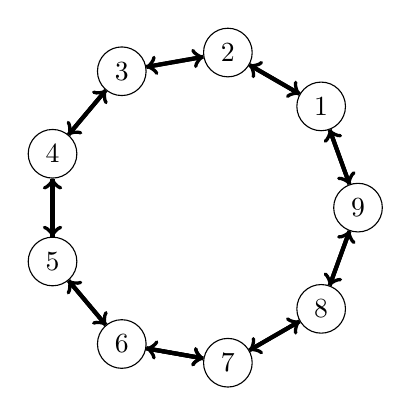
\begin{tikzpicture}
	    \foreach \i in {1,2,...,9}
		\node[circle, draw] (\i) at ({\i*40}:2) {\i};
		
	    \draw[->, line width=1.5pt]  (1) -- (2);
	    \draw[->, line width=1.5pt]  (2) -- (3);
	    \draw[->, line width=1.5pt]  (3) -- (4);
	    \draw[->, line width=1.5pt]  (4) -- (5);
	    \draw[->, line width=1.5pt]  (5) -- (6);
	    \draw[->, line width=1.5pt]  (6) -- (7);
	    \draw[->, line width=1.5pt]  (6) -- (7);
	    \draw[->, line width=1.5pt]  (7) -- (8);
	    \draw[->, line width=1.5pt]  (8) -- (9);
	    \draw[->, line width=1.5pt]  (9) -- (1);
	    \draw[->, line width=1.5pt]  (2) -- (1);
	    \draw[->, line width=1.5pt]  (3) -- (2);
	    \draw[->, line width=1.5pt]  (4) -- (3);
	    \draw[->, line width=1.5pt]  (5) -- (4);
	    \draw[->, line width=1.5pt]  (6) -- (5);
	    \draw[->, line width=1.5pt]  (7) -- (6);
	    \draw[->, line width=1.5pt]  (8) -- (7);
	    \draw[->, line width=1.5pt]  (9) -- (8);
	    \draw[->, line width=1.5pt]  (1) -- (9);
	\end{tikzpicture} 
	\caption{A directed double cycle with only two Hamiltonian cycles and they share no edges in common.}\label{cycles}
\end{figure}
This graph has exactly two Hamiltonian cycles, and technically, they share no edges between them due to the directed nature of the edges. These are the relatively obvious cycles of $(1,2,3,4,5,6,7,8,9)$ and $(1,9,8,7,6,5,4,3,2)$. These are not simple rotations of a solution, they are actually using seperate edges due to the directed nature of the graph. Thus, the 2nd-best solution has no edges in common with the best, or in other words, they are different by a full $|E| = |V|$ edges. So, intuitively no simple method could use the first solution to find the second, as they have nothing in common. If you consider the possibility of this structure being embedded in a larger graph in some manner, it becomes apparent why it might always be computationally difficult  to find the second-best solution even given the best. 

Of course, this was all just to show that \inob{}-TSP is \nph. We must also prove the others. These proofs will be much shorter in this case.

\begin{theorem}
    \exob{}-TSP is $\nph{}$.
\end{theorem}

This proof follows nearly directly from the proof that \inob{}-TSP is $\nph{}$. Due to this, we will omit some details by simply referring to the previous proof. We will still reduce from the original traveling salesman problem.

\begin{proof}
    On an instance of the traveling salesman problem with input graph $G = (V,E)$, we will perform the exact operation used to show the hardness of \inob{}-TSP, with one alteration. In the third step, we perform the following action:
    
    For every edge $(u_1,u_2) \in E$, we create an edge from $H_{u_4}$ to $H_{u_3}$ with weight $w(u_1,u_2) + 1$ (rather than just $w(u_1,u_2)$).

    First, note that an addition of a constant number to all edges in a graph $G$ leaves the solution to the traveling salesman problem unchanged. Notice that performing this modification still allows us to create the tour $T$ with weight zero, it just increases the weight of $T'$ by the number of edges. Finally, it is clear that all of our logic for \inob{}-TSP still holds, except that we now know that the second-best solution will have non-zero weight, thus ensuring that it is strictly worse than the optimal solution. Thus, \exob{}-TSP is also hard.
\end{proof}

Finally, there is one proof remaining. This one is the most obvious of all.
\begin{theorem}
    \exb{}-TSP is $\nph{}$.
\end{theorem}

To prove this problem, we will instead prove the more general result:
\begin{theorem}
\label{exbhard}
    If the \exob{} version of a problem is $\nph{}$, then the \exb{} version must also be.
\end{theorem}

Let $A$ be a general combinitorial optimization problem for which \exb{}-A and \exob{}-A are well-defined. We will reduce from \exob{}-A to \exb{}-A.

\begin{proof}
    On an instance of \exob{}-A with input graph $I$ and provided optimal solution $S$, we create an instance of \exb{}-A with the input $I$ and nothing else. By definition, the solution to \exb{}-A must also be a solution to \exob{}-A, as it aims to find the same answer just with less information. Clearly, this reduction runs in polynomial time. Thus, this is sufficient to show that \exb{}-A is \nph.
\end{proof}

This result is unsurprising, as it is difficult to imagine a situation in which it is harder to find the second-best solution simply because you were given \textit{more} information.

Thus, every possible second-best version of the traveling salesman problem on unrestricted graphs is $\nph{}$. A slightly sad, if potentially expected result due to the computational difficulty of the original problem.

\section{Metric Space TSP}
We showed that the unrestricted version of the traveling salesman problem is hard, but that doesn't tell the full story. There are several well-studied restrictions on the original problem that make it computationally easier. One such restriction is that in which the edge weights of the input graph must satisfy the requirements of a Metric space. That is, the graph must be connected, symmetric (undirected), and the weights of the edges must satisfy the triangle equality. The triangle equality is the following condition: for any three vertices $u,v,x \in V$, $w(u,v) \leq w(u,x) + w(x,v)$. In this case, it becomes possible to create a polynomial-time approximation that is slightly better than a 3/2 approximation \cite{karlin2023slightly, christofides1976worst}. The most famous example of a metric space is the Euclidean space, the space which best defines the world around us. 

We consider whether finding a second-best solution under this new restriction is still difficult.
\begin{theorem}
    \inob{}-Metric-TSP is $\nph{}$
\end{theorem}
This proof is interesting not only for its own details, but also for the fact that we will use a problem that we have proven in this thesis, rather than one that was proven previously, to show this new problem is $\nph{}$. This should be some evidence that our work here will benefit future research in the field. We will reduce from \inob{}-TSP. In particular, we will reduce from \inob{}-Complete-Undirected-TSP, in which the input graph is symmetric and every vertex neighbors every other vertex. As we previously mentioned, \inob{}-Undirected-TSP must be in $\nph{}$, but we do have to briefly prove that requiring completeness doesn't change anything.

\begin{lemma*}
    \inob{}-Complete-Undirected-TSP is $\nph{}$
\end{lemma*}
We will reduce from \inob{}-Undirected-TSP 
\begin{proof}
    On an instance of \inob{}-Undirected-TSP with input graph $G = (V,E)$, weights defined by $w$, and provided optimal tour $T$, we craft $G' = (V',E')$, $w'$, and $T'$ as follows:
    \begin{enumerate}
        \item First, we set $V' = V$, the set of vertices is unchanged.
        \item Let $M = \max_{u,v\in V}[w(u,v)]$, the maximum edge weight between any two vertices in $V$.
        \item For every edge $(u,v)\in E$, we put $(u,v)$ in $E'$ with the same weight.
        \item For every pair of vertices $x,y \in V$ such that $(x,y) \not \in E$, we put $(x,y)$ in $E'$ with the weight $w'(x,y) = |V| * M + 1$.
        \item We set $T' = T$
    \end{enumerate}

    First, we must prove that $T'$ is still an optimal tour in $G'$. First, clearly is is a Hamiltonian cycle as the set of vertices hasn't changed and every edge in $E$ is also in $E'$. Suppose towards a contradiction that there is a Hamiltonian cycle $T''$ in $G'$ such that $w(T'') < w(T')$. Thus, there must be some edge $e$ in $T''$ that is not in $T'$. This edge can either be an edge from step (3) or an edge from step (4). If $e$ is from step (4), then $w(e) = |V| * M + 1$. Note that the number of edges in any Hamiltonian cycle in $G'$ must be exactly $|V|$. Since $T' = T$, it must include only edges that are originally in $G$, the maximum possible edge weight present in $T'$ would be $M$. Thus, the maximum possible total weight of $T'$ is $|V|*M$, less than $w(e)$. Thus, $e$ cannot be from step (4) while maintaining $w(T'') < w(T') $. However, if $e$ is from step (3), then it must be an edge that is also present in $G$. Since this is true for every edge in $T''$, every edge in $T''$ must also have originally been in $G$. However, since the edge weights of each of these edges is the same in $G'$ as it was in $G$, then $T''$ must be a Hamiltonian cycle of $G$ as well, and must have a lower weight than $T$, since $T = T''$. This contradicts the fact that $T$ is an optimal tour on $G$. Thus, $T'$ is an optimal tour in $G'$.

    Finally, we must show that the solution to \inob{}-Complete-Undirected-TSP on $G'$, $w'$, and $T'$ directly provides the solution to \inob{}-Undirected-TSP.

    Let $T''$ be a solution to \inob{}-Complete-Undirected-TSP. By the same logic as in our proof of the optimality of $T'$, we know that exactly one of the following must be true:
    \begin{itemize}
        \item $T''$ includes no edges from step (4).
        \item There is no second Hamiltonian cycle in $G$.
    \end{itemize}
    This is because \textit{any} Hamiltonian cycle that includes only edges in $G$ will have a maximum weight of $|V|*M$, whereas if any edges not in $G$ are included that weight immediately explodes to a minimum total weight of $|V|*M + 1$. Thus, any $G$-only tour is better than any tour that includes edges outside of $G$. Thus, if there is no second-best solution that exclusively has edges in $G$, then there is no solution at all to our original problem. On the other hand, if there is a second-best solution that exclusively uses edges in $G$, then clearly that solution will also be the second-best solution to \inob{}-Undirected-TSP, since any theoretically better solution in $G$ would also exist in $G'$ and would have the same, lower total weight in $G'$, which would be a contradiction. Thus, we can use the solution to \inob{}-Complete-Undirected-TSP to immediately solve the original \inob{}-Undirected-TSP, an $\nph{}$ problem. This concludes our proof that \inob{}-Complete-Undirected-TSP is $\nph{}$.
\end{proof}
Finally, this lets us reach the stage where we can proof that \inob{}-Metric-TSP is also $\nph{}$.
\begin{proof}
    On an instance of \inob{}-Complete-Undirected-TSP with input graph $G = (V,E)$ with edge weights $w$ and provided optimal tour $T$, we create the following $G' = (V', E')$ with edge weights $w'$:
    \begin{enumerate}
        \item We set $V' = V$, remaining unchanged.
        \item Calculate $M = \max_{u,v\in V}[w(u,v)]$, the maximum edge weight between any two vertices in $V$.
        \item For every vertex pair $u,v \in V$, set $w'(u,v) = w(u,v) + M$ in $E'$.
    \end{enumerate}
    Note that all of the above steps are easily achieved in polynomial time.
    First, we must ensure that the new graph we have created is in fact a metric space. Clearly, the graph is complete -- every vertex shares an edge with every other vertex. So, we must show that the triangle inequality is maintained. Let $u,v,x$ be three arbitrary vertices in $V'$. Then,
    \begin{equation*}
    \begin{split}
              w'(u,v) &= w(u,v) + M  \\
        &\leq M + M \\
        &\leq w(u,x) + M + w(x,v) + M\\
        &= w'(u,x) + w'(x,v)
    \end{split}
    \end{equation*}
    Thus, $G'$ satisfies the triangle inequality and is a valid metric space.
    
    As we noted in our proof that \exob{}-TSP is $\nph{}$, adding a constant to the weight of all edges in a graph clearly does not change the order of the lowest weight Hamiltonian cycles. Looking back at our construction of $G'$, that is exactly what we did, simply adding a constant to every edge weight. Thus, we have effectively shown that a solution to \inob{}-Metric-TSP on $G'$ must be exactly a solution to \inob{}-Complete-Undirected-TSP.  This concludes the proof that \inob{}-Metric-TSP is $\nph{}$
\end{proof}

We aren't quite done with Metric TSP until we've examined the other second-best options.
\begin{theorem}
    \exob{}-Metric-TSP is $\nph{}$
\end{theorem}
For this proof, as one might expect, we will reduce from \inob{}-Metric-TSP.
\begin{proof}
    On an instance of \inob{}-Metric-TSP with complete input graph $G = (V,E)$, weight function $w$, and provided optimal solution $T$, we create a $G' = (V',E')$, $w'$, and $T'$:
    \begin{enumerate}
        \item Let $V' = V$.
        \item Calculate $M = \max_{u,v\in V}[w(u,v)]$, the maximum edge weight between any two vertices in $V$.
        \item Calculate $L = \min_{u,v,x,y\in V}[|w(u,v) - w(x,y)|]$, the minimum difference in edge weights between any two edges in $E$.
        \item For every edge $e \in E$ that is not in $T$, add $e$ to $E'$ but set $w'(e) = w(e) + 3M + 1$. 
        \item For every edge $e$ that is in $T$, add $e$ to $E'$ with edge weight $w'(e) = w(e) + 3M + 1 - \frac{L}{|V|^2}$.
        \item Let $T' = T$
    \end{enumerate}
    
    First, we must show that this new graph is also metric. Let $u,v,x \in V'$. Then,     
    \begin{equation*}
    \begin{split}
              w'(u,v) &\leq w(u,v) + 3M + 1  \\
        &\leq M + 3M + 2  = 4M + 2 \\
        &\leq w(u,x) + 2M + 1 + w(x,v) + 2M + 1\\
        &\leq w(u,x) + (3M- \frac{L}{|V|^2}) + 1 + w(x,v) + (3M- \frac{L}{|V|^2}) + 1 \\
        &\leq w'(u,x) + w'(x,v)
    \end{split}
    \end{equation*}
    
    Thus, $G'$ satisfies the triangle inequality.
    
    Additionally, clearly $T'$ is still optimal in $G'$, since all the edges not in $T'$ would have increased more than any of the edges in $T'$ when moving from $E$ to $E'$. So, all that remains to show is that a solution to \exob{}-Metric-TSP on this new input gives us a solution to \inob{}-Metric-TSP. First, we must prove a small lemma.

    \begin{lemma*}
        $T'$ is the one and only optimal solution in $G'$. That is, there is no other Hamiltonian cycle in $G'$ with a weight less than \textit{or} equal to $T'$.
    \end{lemma*}

\begin{proof}
        To prove this lemma, suppose there exists a tour $T''$ in $G$ that has the same total weight as $T$. That is, $w(T'') = w(T)$ In this case, $T''$ is clearly a valid solution to \inob{}-Metric-TSP. Now, if we consider the version of $T''$ in $G'$ instead, first note that $w'(T) = w'(T') = \sum_{e\in T} w(e) + 3M + 1 - \frac{L}{|V|^2}$ whereas $w'(T'') = \sum_{e\in T} w(e) + 3M + 1 $. Since $\frac{L}{|V|^2}$ is always positive, that means that $w'(T'') > w'(T)$. This is the key change, as it enables us to say confidently that $T'$ is the one and only optimal solution for graph $G'$, and any other solution is strictly worse.
\end{proof}
    To complete our proof that \exob{}-Metric-TSP is $\nph{}$, we show that $T''$ is an inclusive second-best solution in $G$ $\iff$ $T''$ is an exclusive second-best solution in $G'$.
    ($\Rightarrow$) Suppose $T''$ is an inclusive second-best solution in $G$. That is, $w(T'') \leq w(C)$ for any Hamiltonian cycle $C \neq T$ in $G$. Now, suppose towards a contradiction that there is a Hamiltonian cycle $C \neq T'$ in $G'$ such that $w'(C) < w'(T'')$. 
    Let us consider the weight of $C$ in the original graph $G$. Since neither $C$ nor $T'' $are the optimal tour in $G'$, they both must contain at least one edge that is not in $T'$. By our construction of $G'$, this means that:
\begin{equation*}
\begin{split}
w'(C) &> w(C) + 3M + 1 - |V|*\frac{L}{|V|^2}\\
 &= w(C) + 3M + 1 - \frac{L}{|V|}
\end{split}
\end{equation*}
and
\begin{equation*}
\begin{split}
w'(T'') &\leq w(T) + 3M + 1\\
\end{split}
\end{equation*}
Since we have assumed that $w'(C) < w'(T'')$, these two inequalities imply that 
\begin{equation*}
\begin{split}
w(C)  &< w(T) + \frac{L}{|V|}\\
\end{split}
\end{equation*}
However, since we defined $L$ as the smallest difference between any two edge weights in $G$, it is impossible for it to be the case that $w(T'') \leq w(C) <  w(T'') + \frac{L}{|V|}$. Thus, it must also be the case that $w(C) \geq w(T'') + \frac{L}{|V|} $. From our above equations, we know that this also means that $w'(C) \geq w'(T'')$. This contradicts our assumption that $w'(C) < w'(T'')$. Therefore, by contradiction, $T''$ must be a second-best solution in $G'$. By our lemma above, we also know that $w'(T'') > w'(T')$, making $T''$ an exclusive second-best solution. 

($\Leftarrow$) Now suppose $T''$ is an exclusive second-best solution in $G'$. That is, $w'(T') < w'(T'') < w'(C)$ for any Hamiltonian cycle $C \neq T', C \neq T''$ in $G'$. Consider any Hamiltonian cycle $D \neq T,D\neq T''$ in $G$. By our construction of $G'$, we have:

\begin{equation*}
\begin{split}
w(D) &\geq w'(D) - 3M - 1 \\
&> w'(T'') - 3M - 1 \\
&\geq w(T'') - \frac{L}{|V|}
\end{split}
\end{equation*}
However by the same logic we used in the previous direction, we know that $w(D)$ cannot be between $w(T'')$ and $w(T'')-\frac{L}{|V|}$. Thus, $w(D) \geq w(T'')$, concluding our proof that $T''$ must be an inclusive second-best solution in $G$.

This completes the proof that $T''$ is an inclusive second-best solution in $G$ if and only if $T''$ is an exclusive second-best solution in $G'$. Since \inob{}-Metric-TSP is NP-hard and we have shown a polynomial-time reduction from \inob{}-Metric-TSP to \exob{}-Metric-TSP, we can conclude that \exob{}-Metric-TSP is also NP-hard.
\end{proof}

Finally, of course:
\begin{theorem}
    \exb{}-Metric-TSP is $\nph{}$
\end{theorem}
This follows immediately from our \autoref{exbhard}.

\section{Euclidean Graph TSP}
In the section on metric TSP, we mentioned one particularly common example of a metric space, that of Euclidean space. Many of the real-world applications of TSP are not acting on completely arbitrary graphs, or even non-Euclidean metric graphs. Rather, they act on graphs that closely or exactly resemble the Euclidean space we are familiar with. We can restrict the traveling salesman problem to exist only on the Euclidean plane -- that is a complete, undirected graph where the weight of an edge between two points is the Euclidean distance between them. 

The question of single-best optimality has itself been well-studied, with interesting results outside of the study of the second-best. One key result to note is that, unlike the unrestricted and metric versions, Euclidean TSP permits a polynomial time approximation scheme, or an approximation algorithm with arbitrary accuracy. Sadly, despite this approximability, we have found that Euclidean TSP is still hard in all second-best forms. In other words, it is \exobht{}, \inobht{}, and of course therefore \exbht{}. We sat with this problem for a considerable amount of time, not sure which direction it would go. Initially, we suspected that the comparitive ease of approximating Euclidean TSP would lead to finding the second-best solution being possible. Thus, we attempted to develop intuition regarding the problems using example graphs. We include some of our examples below, in which we checked how far the first and second-best solutions were from each other in terms of their differences of edges as well as their total weight.



In the first example \autoref{9points}, we discovered a graph with 5 vertices in which the first and second-best solutions differ by 4 edges, and thus share only one. We found it difficult to generalize this graph to larger values of $|V|$, but it hints that Euclidean graphs can still have very high edge differences between the top solutions. Like our graph in \autoref{cycles} did for the unrestricted form of TSP, this implies there is no brute force conversion from the best to the second-best solution. While this doesn't prove hardness, it did help inform our further steps.
\begin{figure}[!ht]
	\centering
	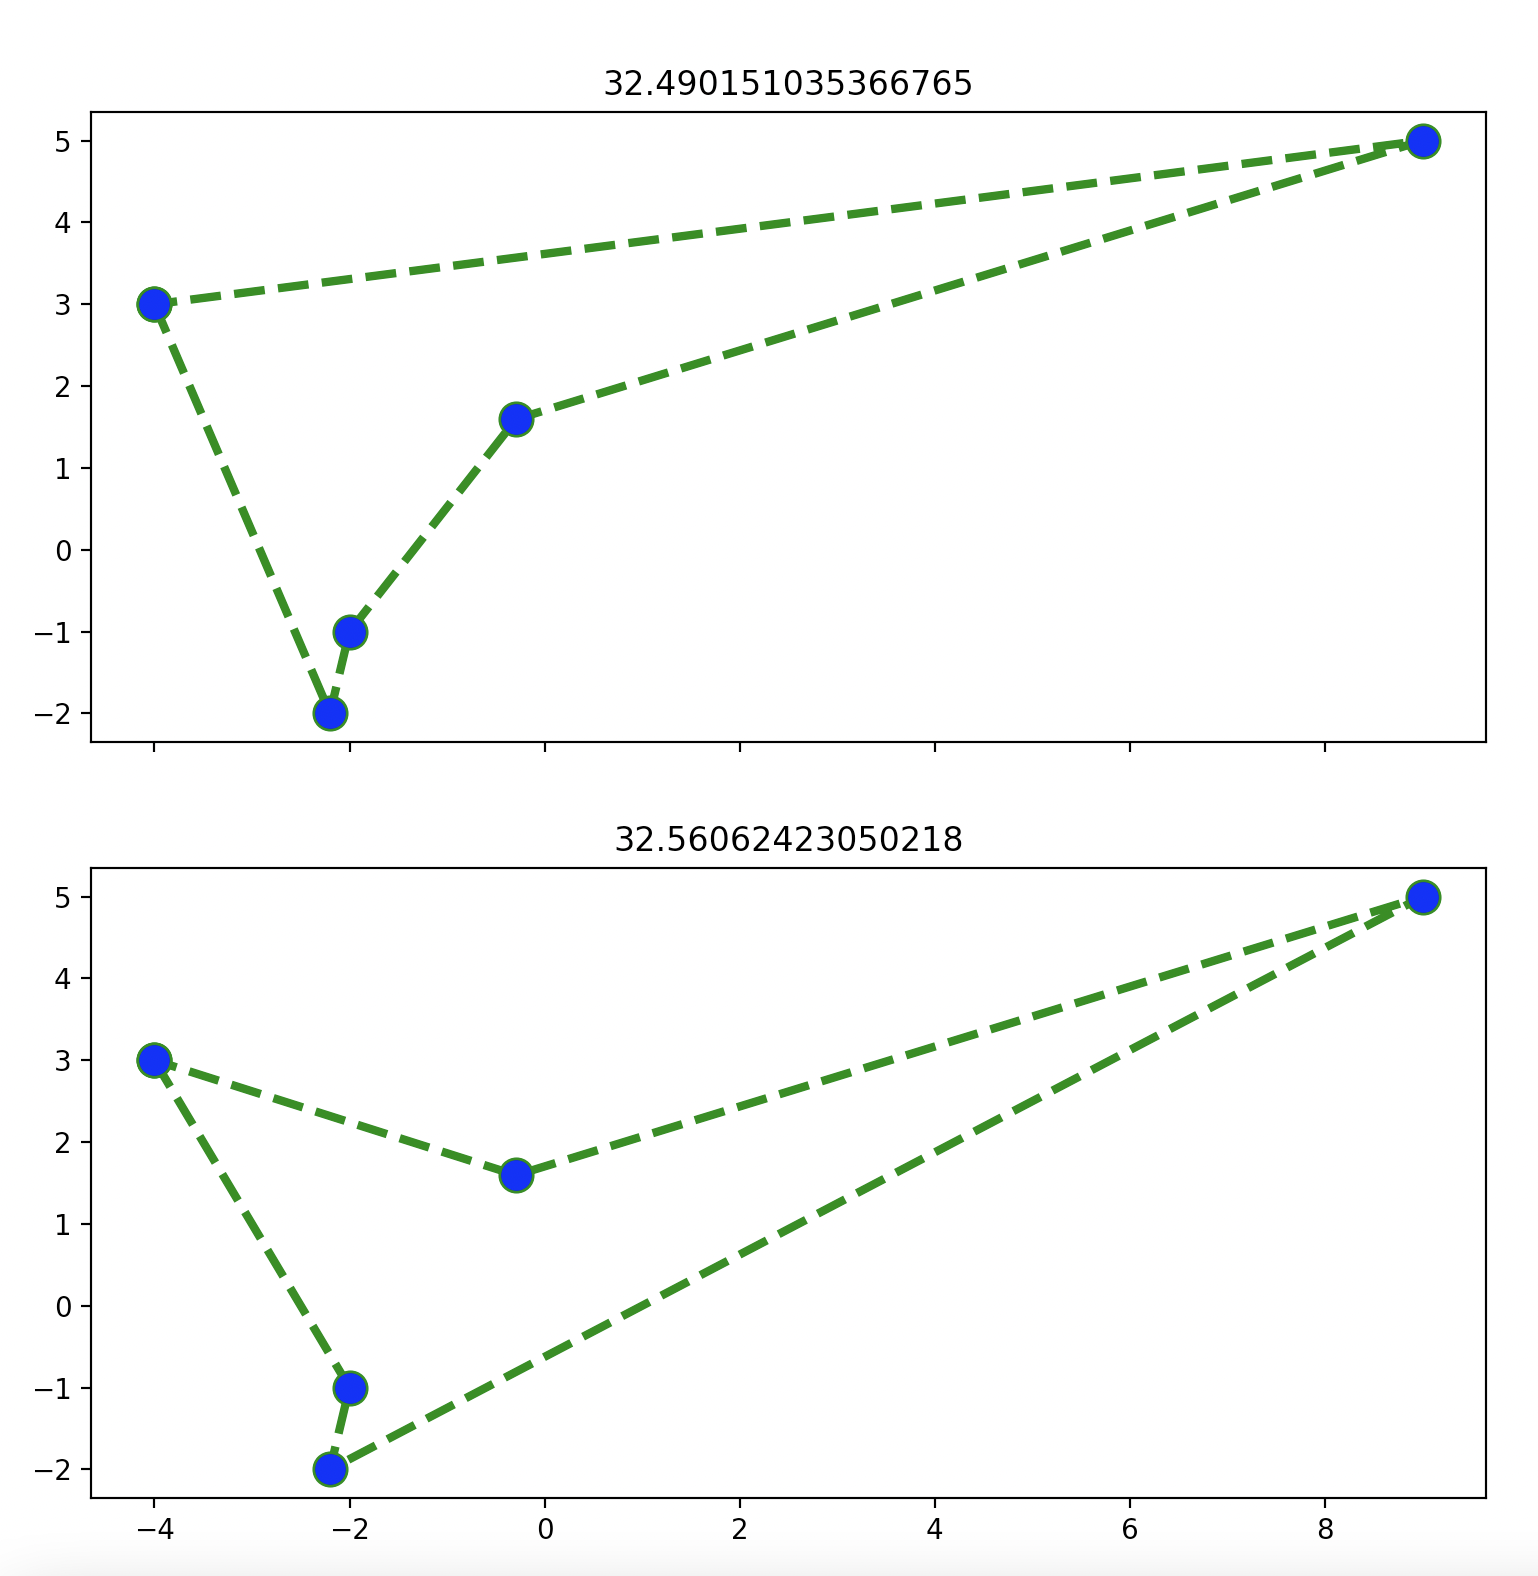
\includegraphics[width=\textwidth, height=.5\textheight, keepaspectratio]{images/5points.png}
	\caption{A Euclidean graph with 5 vertices in which the second-best TSP (bottom) shares only one edge in common with the optimal TSP (top)}\label{5points}
\end{figure}

Another interesting graph comes from the idea of the near-parallel lines mentioned in Rothe \cite{rothe1988two}. The example in \autoref{9points} shows 3 near parallel lines each made of 3 points, and the first and second-best solutions differ by 3 edges. 

\begin{figure}[!ht]
	\centering
	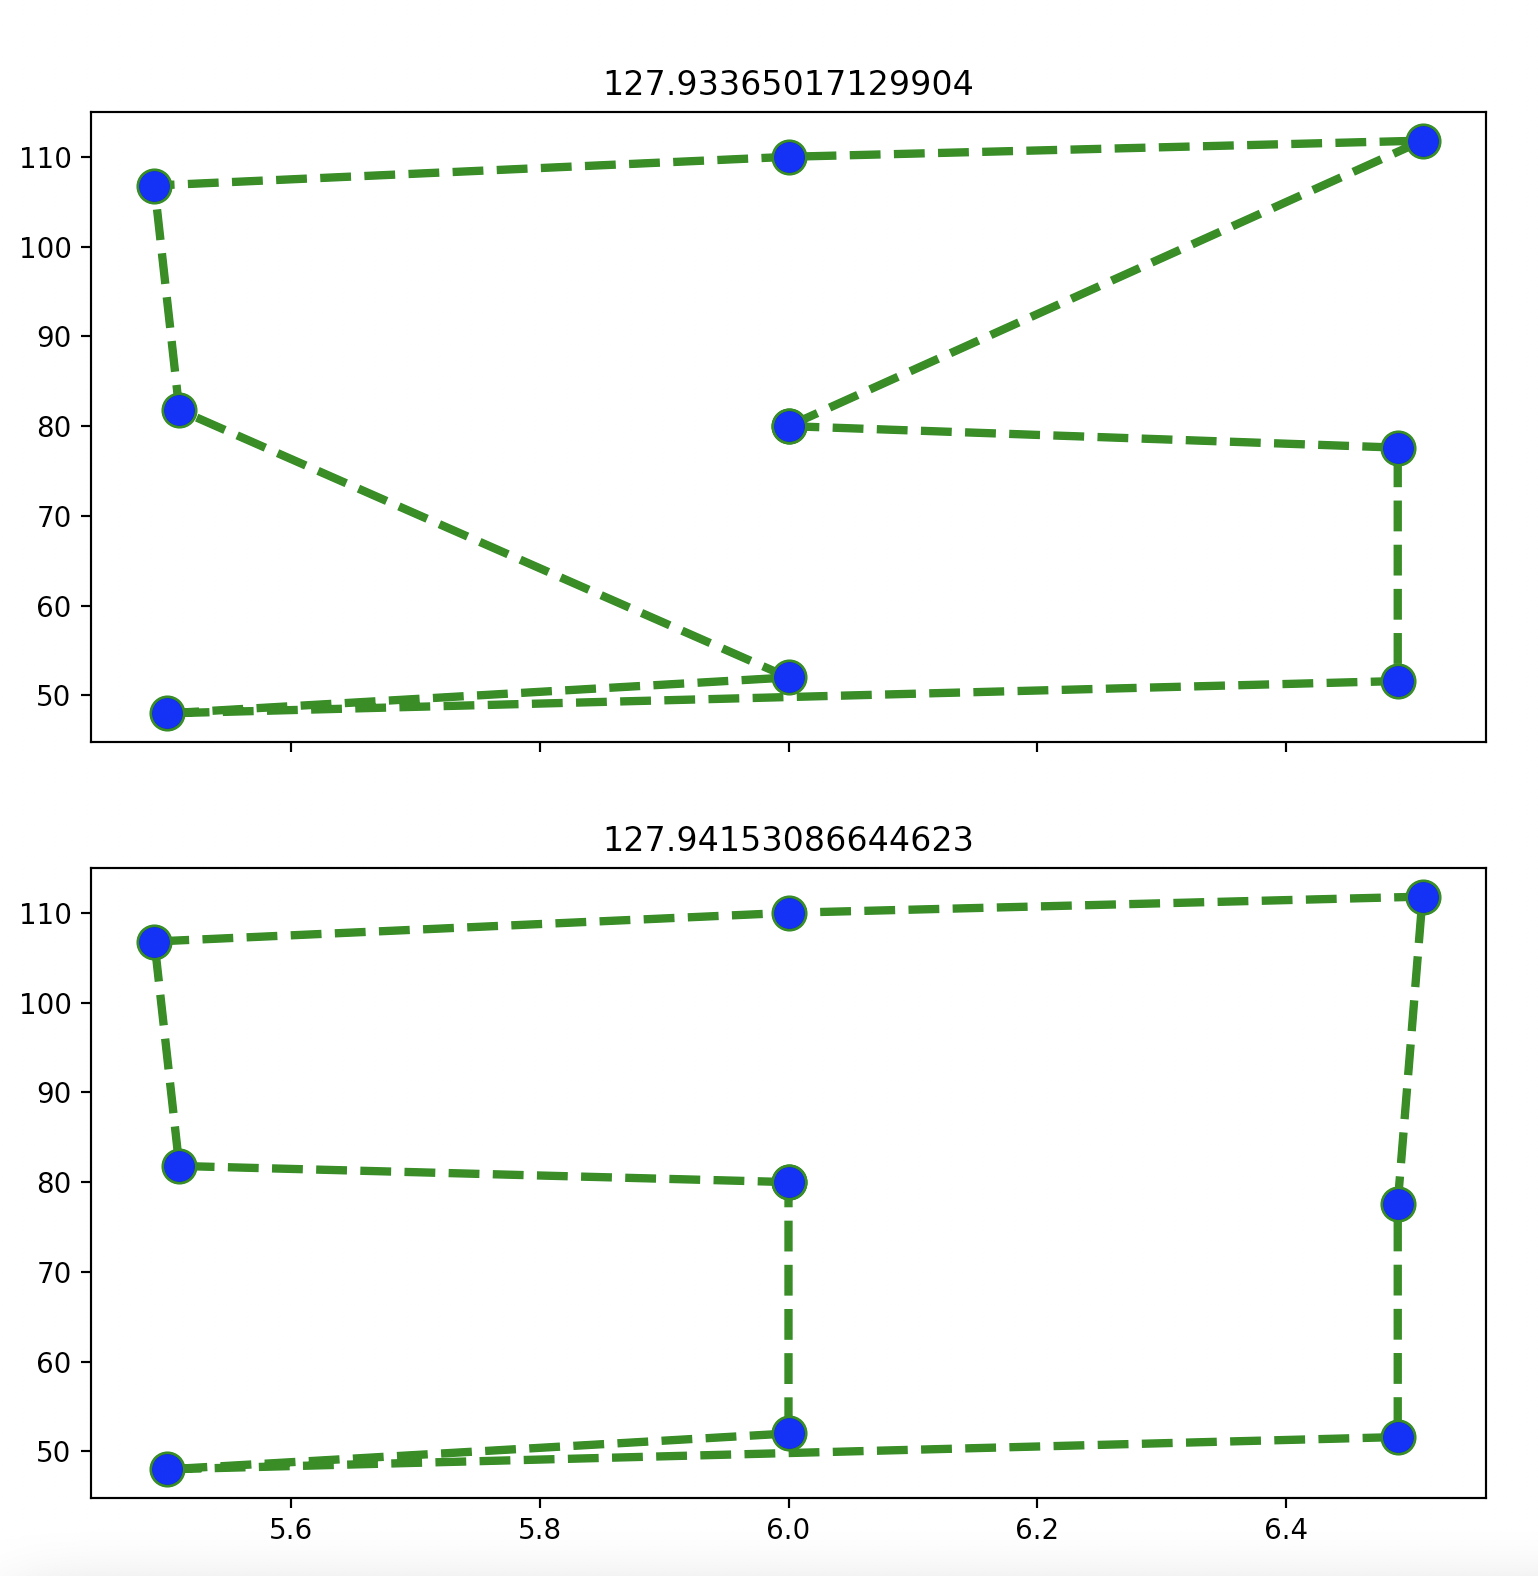
\includegraphics[width=\textwidth, height=.5\textheight, keepaspectratio]{images/9points.png}
	\caption{A Euclidean graph of 3 near-parallel lines with 9 vertices in which the second-best TSP (bottom) differs by 3 edges ($\frac{|V|}{3}$) from the optimal solution (top).}\label{9points}
\end{figure}


We will leave formalizing the second-best Euclidean TSP proofs for future work in the field, however it follows from Papadimitriou's proof of the $\npc{}$ nature of the Euclidean TSP \cite{papadimitriou1977euclidean}. In his proof, he reduces from the $\npc{}$ Exact Cover problem in which the input is a universe set $U$ and a collection of subsets $\mathcal{S}$ of $U$ and the goal is to find a subcollection $\mathcal{C} \subseteq \mathcal{S}$ in which every element in $U$ is contained in exactly one subset of $\mathcal{C}$. By creating a very specific set of Euclidean subgraphs, he is able to force a minimum Hamiltonian cycle of a certain weight if and only if there is an exact cover of the input set.

Our modification to this proof would be relatively simple compared to the proof itself. Originally, Papadimitriou uses his construction to prove that Euclidean path-TSP, rather than cycle, is NP-Complete. To show that the Euclidean tour-TSP, what we would refer to simply as Euclidean TSP, is $\npc{}$, he connects the start and endpoint with his 1-chain construction to force an optimal solution to go directly from the latter back to the former at the end of the loop. Instead, for \inob{}-Euclidean-TSP we would connect the start and endpoint with his 2-chain construction, giving two equally weighted loops that are the same besides the mode of traversal between the start and endpoint. For \exob{}-Euclidean-TSP, we would do the same, except make one of the modes through the chain a tiny amount worse than the other by moving one of its vertices a small amount to the side. For more details, it is important to read \cite{papadimitriou1977euclidean}. We would expect future work in the field to formalize this proof.


\section{Convex Euclidean TSP}
We will examine one more version of the travelling salesman problem. After it became clear that the other versions of TSP were consistently $\nph{}$, we decided to consider a much heavier restriction on the input graphs than any of the previous problems. In fact, Convex Euclidean TSP is so heavily restricted that the original optimization problem is in P, making it the first problem in the class of P that we examined that was not already studied in terms of second-best solutions. However, the easiness of the original problem does not make the second-best question uninteresting, as it is not immediately apparent whether it will still be easy to find the second-best solution as well. This type of question, asking whether or not computing the optimal solution is actually easier to find than any that come after it, is the basis behind much of the research into $k$-best problems that came before us, but is even more prevalent here as the convex Euclidean version of the travelling salesman problem feels so close to being $\nph{}$. First, let us define what we mean for a graph to be convex. If $G$ is a 2-dimensional Euclidean graph -- as defined in the section above -- in which the points form a convex polygon, then we will show that \exob{}-Convex-Euclidean-TSP and \inob{}-Convex-Euclidean-TSP on $G$ can be solved in polynomial time.  Note the known result that the optimal solution to the traveling salesman problem on a convex Euclidean graph is simply the convex hull of the graph, which is obtainable in polynomial time. This result comes from the proof that the solution to Euclidean TSP must never have crossings, which in the convex case, leads to only a single possible solution (for general Euclidean TSP, there are many non-crossing tours) \cite{quintas1965on, arora1998polynomial}.

First, we will show that the \exob{} and \inob{} versions of the problem are equivalent, assuming we ignore simple loop reversals (allowing loop reversals simply makes \inob{} very easy, as we can always reverse the best solution, whereas \exob{} would remain unchanged). 
\begin{lemma*}
        $T$ is a solution to \inob{}-Convex-Euclidean-TSP $\iff$ $T$ is a solution to \exob{}-Convex-Euclidean-TSP
\end{lemma*}
\begin{proof}
    This proof follows directly from the original proof that Convex-Euclidean-TSP is easy. Any solution other than the convex hull of the graph must have an edge crossing, and any solution with an edge crossing must have a higher total weight than a solution with no edge crossings. Since there is only one convex hull (up to rotation and reversal), this implies that any non-optimal solution is strictly worse than the optimal. Thus, if $T$ is a solution to \inob{}-Convex-Euclidean-TSP, $T$ is a solution to \exob{}-Convex-Euclidean-TSP and vice-versa.
\end{proof}
Thus, we only need to show that one of the two versions are hard, and we will have a proof that all three versions of the second-best problem are hard. We will use a proof by induction on the number of edges different between optimal tour $T$ and any other tour $T'$. Our goal is to show that any tour $T'$ can always be improved by exchanging edges with $T$. We represent tours in ``vertex,edge,vertex...,vertex" edge notation, as in $a_1,a_1a_2,a_2,...,a_na_1,a_1$ but abuse the notation to refer to only the edges in one tour that are not in the other as $T_1 \setminus T_2$.

\begin{theorem}
    Any suboptimal tour $T'$ can be altered to become $T''$ such that $w(T'') \leq w(T')$ exclusively by removing edge crossings in $T'$.
\end{theorem}

\begin{proof}
    
\textbf{\textit{(Base cases):}} \newline
\textbf{\textit{(Case 0 edge crossings):}}

If there are 0 edge crossings within $T'$, then $T' = T$ since the optimal solution to Euclidean TSP is the only solution that has no edge crossings.
\newline\textbf{\textit{(Case 1 edge crossing):}}

If there is 1 edge crossing within $T'$, let the crossing edges be $uv$ and $xy$. Due to the convexity of the graph, we can replace $uv$ and $xy$ with either $ux$ and $vy$ or $uy$ and $vx$, whichever pair doesn't cross. This replacement does not increase the total cost due to the triangle inequality, as shown in \cite{quintas1965on}. After this replacement, we have a new tour $T''$ with 0 edge crossings, which is the optimal tour $T$. This implies that $|T \setminus T'| = 2$, there are exactly two edges in $T'$ that are not in $T$.
\newline\textbf{\textit{(Inductive Step):}} Suppose that for any Hamiltonian cycle $T'$ with $k$ edge crossings within itself, we can improve $T'$ by replacing crossing edges. We will show that this must also hold for a tour $T'$ with $k+1$ edge crossings.

Let $T'$ be a tour with $k+1$ edge crossings within itself. Choose any pair of crossing edges $uv$ and $xy$. As in the base case with 1 crossing, we can replace these edges with either $ux$ and $vy$ or $uy$ and $vx$, whichever pair doesn't cross, without increasing the total cost. This replacement must always yield a new tour $T''$ with at most $k$ edge crossings. By the inductive hypothesis, we can improve $T''$ -- or at least not make it worse -- by replacing crossing edges until we reach the optimal tour $T$. Since this process is not immediately intuitive, we include an example graph in \autoref{3diff}.

\begin{figure}[!ht]
	\centering
	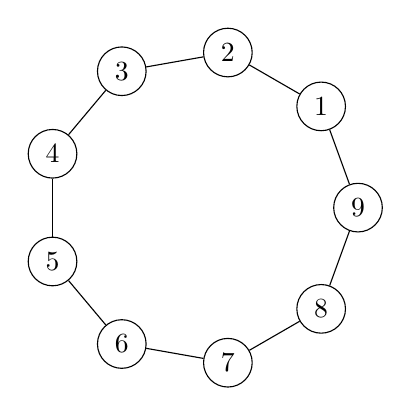
\begin{tikzpicture}
	    \foreach \i in {1,2,...,9}
		\node[circle, draw] (\i) at ({\i*40}:2) {\i};
	    \draw (1) -- (2);
	    \draw (2) -- (3);
	    \draw (3) -- (4);
	    \draw (4) -- (5);
	    \draw (5) -- (6);
	    \draw (6) -- (7);
	    \draw (7) -- (8);
	    \draw (8) -- (9);
	    \draw (9) -- (1);
	\end{tikzpicture} 
	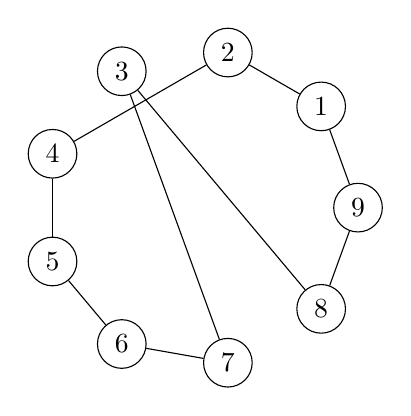
\begin{tikzpicture}
	    \foreach \i in {1,2,...,9}
		\node[circle, draw] (\i) at ({\i*40}:2) {\i};
		
	    \draw (1) -- (2);
	    \draw (2) -- (4);
	    \draw (3) -- (7);
	    \draw (4) -- (5);
	    \draw (5) -- (6);
	    \draw (6) -- (7);
	    \draw (3) -- (8);
	    \draw (8) -- (9);
	    \draw (9) -- (1);
	\end{tikzpicture}
	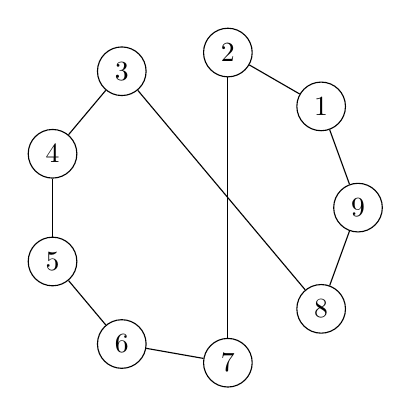
\begin{tikzpicture}
	    \foreach \i in {1,2,...,9}
		\node[circle, draw] (\i) at ({\i*40}:2) {\i};
		
	    \draw (1) -- (2);
	    \draw (3) -- (4);
	    \draw (2) -- (7);
	    \draw (4) -- (5);
	    \draw (5) -- (6);
	    \draw (6) -- (7);
	    \draw (3) -- (8);
	    \draw (8) -- (9);
	    \draw (9) -- (1);
	\end{tikzpicture}
	\caption{An example of the original best tour $T$ (left), a tour $T'$ with $|T \setminus T'| = 3$ (middle), and an example of a tour converted from two edge crossings to one, and $|T \setminus T'| = 3$ to $|T \setminus T'| = 2$ (right)} \label{3diff}
\end{figure}

From our work above, we know that for any suboptimal tour $T'$, we can improve it by repeatedly replacing crossing edges within the tour until we reach the optimal tour $T$. If we stop the process when there is one crossings left, we will have a tour $T''$ such that $|T \setminus T''| = 2$. Since any further decrease in edge crossings would lead to simply finding the optimal solution, that implies that any second-best solution must have $|T \setminus T''| = 2$. Since the number of edges in a complete undirected graph is $\frac{|V|*(|V|-1)}{2}$, that means the number of pairs of edges is 
\begin{equation*}
    \binom{\frac{|V|*(|V|-1)}{2}}{2} = \frac{1}{2}(\frac{|V|*(|V|-1)}{2})(\frac{|V|*(|V|-1)}{2} - 1)
\end{equation*}
which is polynomial in the number of vertices. Thus, finding the second-best tour can be done in polynomial time. We can simply loop through all pairs of edges and check the total weight of a tour that includes those two edges instead of the normal ones in $T$. To determine which edges must be removed for in each case, we can simply also loop through all pairs of edges in $T$, which is $|V|*|V-1|$, and check whether that edge swap would result in a valid Hamiltonian cycle and if it was the best replacement to make. Thus, the total running time of this algorithm is $O(|V|^6)$, which, while a very large polynomial, is still polynomial. Thus, the \exob-Euclidean-Convex-TSP is in complexity class P, as are \inob{}-Euclidean-Convex-TSP and of course \exb{}-Euclidean-Convex-TSP.\end{proof}
There are clearly many ways to improve this algorithm and this solution seems hardly better than brute-force. However, our goal for now was simply to prove that the problem was solvable in polynomial time. We suspect that future work in the area can bring this complexity down to at $O(|V|^2)$ or maybe even $O(|V|)$, making it much more usable in real-world applications. Additionally, this result begs the question of what happens to the complexity of the problem with higher values of $k$ than 2? We suspect that, for a polynomial $k$, it should still be polynomial to find the $k$-th best solution following the same logic as above, since it should have at most $k$ edge-crossings. However, we will leave the proof of this to further research.





% The Traveling Salesman Problem, or TSP is a widely studied {NP-Hard} combinitorial optimization problem in which the decision version of the problem is {{NP-Hard}}. There are three commonly referenced versions of the problem.
% \section{Euclidean TSP}
% \subsection{Standard Euclidean TSP}
% \hfill\\
% If we restrict the traveling salesman problem to exist only on the Euclidean plane, or in other words, every 'city' is a point on the 2D Euclidean plane and every 'route' between two cities is the Euclidean distance between the two points, we are able to slightly limit the likely solution set. This leads to interesting results in general with Euclidean TSP, including that it permits a polynomial time approximation scheme, or an approximation algorithm with arbitrary accuracy. However, despite this approximability, Euclidean TSP is still hard in all second-best forms. In other words, it is \exobht{}, \inobht{}, and of course therefor \exbht{} and \inbht{}. This is the last time we will explicitly mention a problem being \exbht{} and \inbht{}, as any \exobht{} or \inobht{} problem must also be \exbht{} and \inbht{}, and any {NP-Hard} problem is also \exbht{} and \inbht{}. We also develop some geometric intuition for why this may be the case using example graphs.
% \subsection{Convex Shape TSP}
% \hfill\\
% If we further restrict the input graph for the problem to be a convex shape on the Euclidean plane, or in other words the input graph could be represented as a convex polygon, then the problem becomes easier. It is previously proven that finding the optimal (first best) solution for this problem is in {P}. However, it is not obvious that \exobt{{-Convex-TSP}} or \inobt{{-Convex-TSP}} are quite as easy. We prove both in our results section. 
% \section{Metric TSP}
% If instead of the Euclidean distance metric being the restriction of route costs, we use a generic metric that satisfies the triangle inequality, TSP becomes even more difficult. In this case, we lose the polynomial-time-approximation scheme, but it is still possible to create a polynomial-time approximation that is slightly better than a 3/2 approximation. Similarly to the Euclidean case, Metric TSP is both \exobht{} and \inobht{}.
% \section{General TSP}
% In the case where there are no restrictions on the cost to travel between two cities, the traveling salesman problem becomes much harder. In this case, there are no approximations with constant or arbitrary accuracy. Unsurprisingly, the general Traveling Salesman Problem is \exobht{} and \inobht{}.